% Add option "final" for final Master thesis
\documentclass[utf8]{stageM2R}
\usepackage{graphicx}
\usepackage{float}
\usepackage{hyperref}
\usepackage[T1]{fontenc}
\usepackage[french]{babel}

\author{Thibault de \textsc{Villèle}}
%% encadrants
\supervisors{Noura \textsc{Faraj}\\Christophe \textsc{Fiorio}\\Benjamin \textsc{Charlier}}
\location{LIRMM UM5506 - CNRS, Université de Montpellier}
\title{Gestion, traitement et visualisation d'images médicales à très haute résolution}
\track{IMAGINA}
\date{\today}
\version{6}
\abstractfr{
	Lors de la deuxième année de Master en Informatique, nous pouvons effectuer un stage de recherche parmi les sujets proposés dans les laboratoires de recherche. Le sujet de stage choisi est le fruit d'une collaboration entre l'Université de Tulane (Tulane University, La Nouvelle Orléans, États-Unis) et le LIRMM. Ce rapport présente une étude préliminaire sur les modalités de reconstruction tridimensionnelle d'un ensemble d'images médicales à très haute résolution, et de la visualisation de celles-ci. Le but est de proposer un programme de visualisation et de traitement de ces images médicales à très haute résolution. Dans cette étude, nous allons tout d'abord voir les spécificités du système d'acquisition microscopique des images, les problèmes de la méthode déjà en place, puis nous allons tenter de résoudre le problème de la reconstruction 3D, ainsi que donner une piste de résolution afin de visualiser en temps réel les images obtenues.
}

\begin{document}
	\selectlanguage{french}
	\frontmatter \maketitle
	\cleardoublepage
	\tableofcontents \mainmatter

	\chapter{Introduction au domaine de recherche}\label{section:01_intro}
	{
		\section{Contexte et objectifs}\label{section:01_01_contexte}
		{
			Ce stage de recherche, encadré par Mme \textsc{Faraj}, M.\textsc{Fiorio} tous deux de l'équipe ICAR du LIRMM, ainsi que M.\textsc{Charlier} du département de mathématiques de la faculté des sciences de l'université de Montpellier. Ce stage est également en collaboration avec l'université de Tulane, à la Nouvelle Orléans, et a pour but l'amélioration et l'optimisation d'un processus de reconstruction tridimensionnelle d'images médicales à haute résolution.\\

			Actuellement, les diagnostics du cancer de la prostate et les décisions de traitement de celui-ci sont faits à partir d'images histologiques\footnotemark~ 2D~\cite{cite_gleason_use_in_histology_poster}. Les formes des contours des glandes sont comparés à une échelle schématique 2D appelée échelle de Gleason~\cite{cite_gleason_score} afin de déterminer le stade du cancer. La variabilité des plans de coupe peut entraîner un diagnostic et un traitement inadaptés au patient.
			\footnotetext{Image représentant des tissus biologiques, morts ou vivants.}\\

			Nos partenaires chercheurs de l'université de Tulane ont développés une nouvelle méthode d'acquisition de tissus humains de très haute résolution et précision, à l'aide d'un microscope à éclairage sélectif, en utilisant une variation de la méthode \textit{SPIM}~\cite{cite_spim_explication_original}, qui signifie \textit{Single Plane Illumination Microscopy} (voir Chapitre \ref{section:02_description} : \nameref{section:02_description}). Cette méthode permet d'obtenir des séquences d'images numériques précises de l'ordre du micromètre d'un échantillon tridimensionnel transparisé, permettant de voir précisément la formation des cellules du corps humain.\\

			Le but global du projet est d’étudier la morphologie 3D des glandes à l'aide de méthodes de traitement (topologiques et géométriques) et d’une visualisation interactive de données médicales massives issues de la microscopie à éclairage sélectif. Cela permettrait d’enrichir les stratégies de diagnostic du cancer de la prostate existantes.\\

			Plus précisément, l'objectif principal de ce sujet de stage de Master est de proposer un système permettant la visualisation interactive de ces données volumiques massives afin de permettre une première exploration de la forme 3D des glandes de la prostate d'un patient.
		}
		\section{Problématique}\label{section:01_02_problematique}
		{
			Les images en sortie du microscope sont de très haute résolution et très volumineuses (de l'ordre de $2^{34}$ octets). La problématique principale est donc d'imaginer des stratégies spécifiques d’analyse et de visualisation afin de pouvoir visualiser les modèles issus du microscope. En effet, aucune solution actuelle ne permet de visualiser des images médicales de cette taille, et encore moins de les analyser.\\

			Étant donné que le domaine d'activité principal de nos partenaires de Tulane n'est pas la reconstruction 3D, leur méthode de reconstruction des échantillons après acquisition est également à refaire, afin non seulement pour que l'on puisse réduire la taille des grilles 3D résultantes d'une acquisition, mais aussi afin de faciliter la visualisation et le traitement par la suite.
		}
	}

	\chapter{Description de la méthode d'acquisition}\label{section:02_description}
	{
		\section{Acquisition de données}\label{section:02_01_acquisition}
		{
			La microscopie en fluorescence à feuille de lumière~\cite{cite_lsfm_explication_girard} (\textit{Light-Sheet Fluorescence Microscopy}, \textit{LSFM}) est une méthode d'acquisition d'images qui consiste à illuminer une fine tranche de l'échantillon à analyser perpendiculairement à l'axe du système de détection du microscope. La méthode utilisée par les chercheurs de l'université de Tulane est une variation d'une méthode de \textit{LSFM} appelée \textit{SPIM} : \textit{Single Plane Illumination Microscopy}, ou microscopie par éclairage sélectif en français. Cette méthode permet de faire des acquisitions par pile d'images rapidement, et permettant une reconstruction 3D d'un échantillon. Afin d'effectuer une acquisition avec un microscope \textit{SPIM}, l'échantillon a d'abord besoin d'être rendu transparent. En effet, la méthode \textit{SPIM} repose sur l'éclairage latéral d'une partie de l'échantillon, perpendiculairement à l'axe d'acquisition, ce qui rend les dispositifs d'acquisition et de détection complètement indépendants l'un de l'autre.\\

			\begin{figure}[H]
				\centering
				
\includegraphics[width=0.5\linewidth]{./img/lsm_methode_01.jpg}
				\caption{Processus d'acquisition par \textit{SPIM} : un rayon lumineux (en bleu) est envoyé dans l'échantillon, et la fluorescence de celui-ci est détectée par le dispositif de détection dans sa zone focale (en jaune)}
				\label{img:lsm_01_how_it_works}
			\end{figure}

			Par rapport à d'autres techniques de microscopie 3D, la méthode \textit{SPIM} offre les avantages de s’adapter à l'observation d’échantillons en statique et en dynamique (imagerie 4D). Elle permet alors d’observer des organismes transparents vivants (racines, plancton, poisson zèbre, embryons...) mais aussi de remplacer les techniques d’histologie standard (coupes histologiques fines) par l'acquisition en microscopie de tissus clarifiés et/ou transparents.\\

			Dû au fait que les acquisitions sont faites grâce à des émissions de lumière dans l'échantillon à analyser, un problème se présente : l'image d'un point de l'échantillon dans l'acquisition devient une tâche, ceci est dû au phénomène de diffraction de la lumière dans le milieu d'acquisition. Cela entraîne une anisotropie\footnote{L'anisotropie entraîne des propriétés différentes selon des directions différentes (ici, une fonction d'étalement de point différente selon la direction axiale que latérale)} dans l'acquisition 3D d'un échantillon avec la méthode \textit{SPIM} comme on peut voir dans la comparaison des fonctions d'étalement de point\footnote{La fonction d'étalement d'un point est une fonction définissant la réponse d'un système d'imagerie à une source ponctuelle\label{fn:psf}} (figure \ref{img:spim_01_point_spread_function}). Pour pallier à ce problème, on peut effectuer plusieurs acquisitions à des points de vue différents, et c'est la méthode qu'ont choisie les chercheurs de la Nouvelle Orléans pour concevoir leur microscope.\\

			\begin{figure}[!htp]
				\centering
				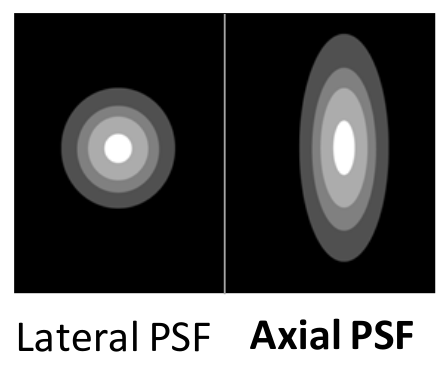
\includegraphics[width=0.3\linewidth]{./img/spim_01_psf.png}
				\caption{Une image des fonctions d'étalement de point (PSF) axiales et latérales en imagerie SPIM}
				\label{img:spim_01_point_spread_function}
			\end{figure}

			Leur variation de la méthode est appelée \textit{diSPIM}, pour \textit{dual inverted SPIM}. Cette variation consiste à utiliser en tandem deux dispositifs \textit{SPIM} afin d'éliminer l'anisotropie qui existe avec les méthodes de \textit{SPIM} traditionnelles (comme vu dans la figure \ref{img:spim_01_point_spread_function}).\\

			\begin{figure}[H]
				\centering
				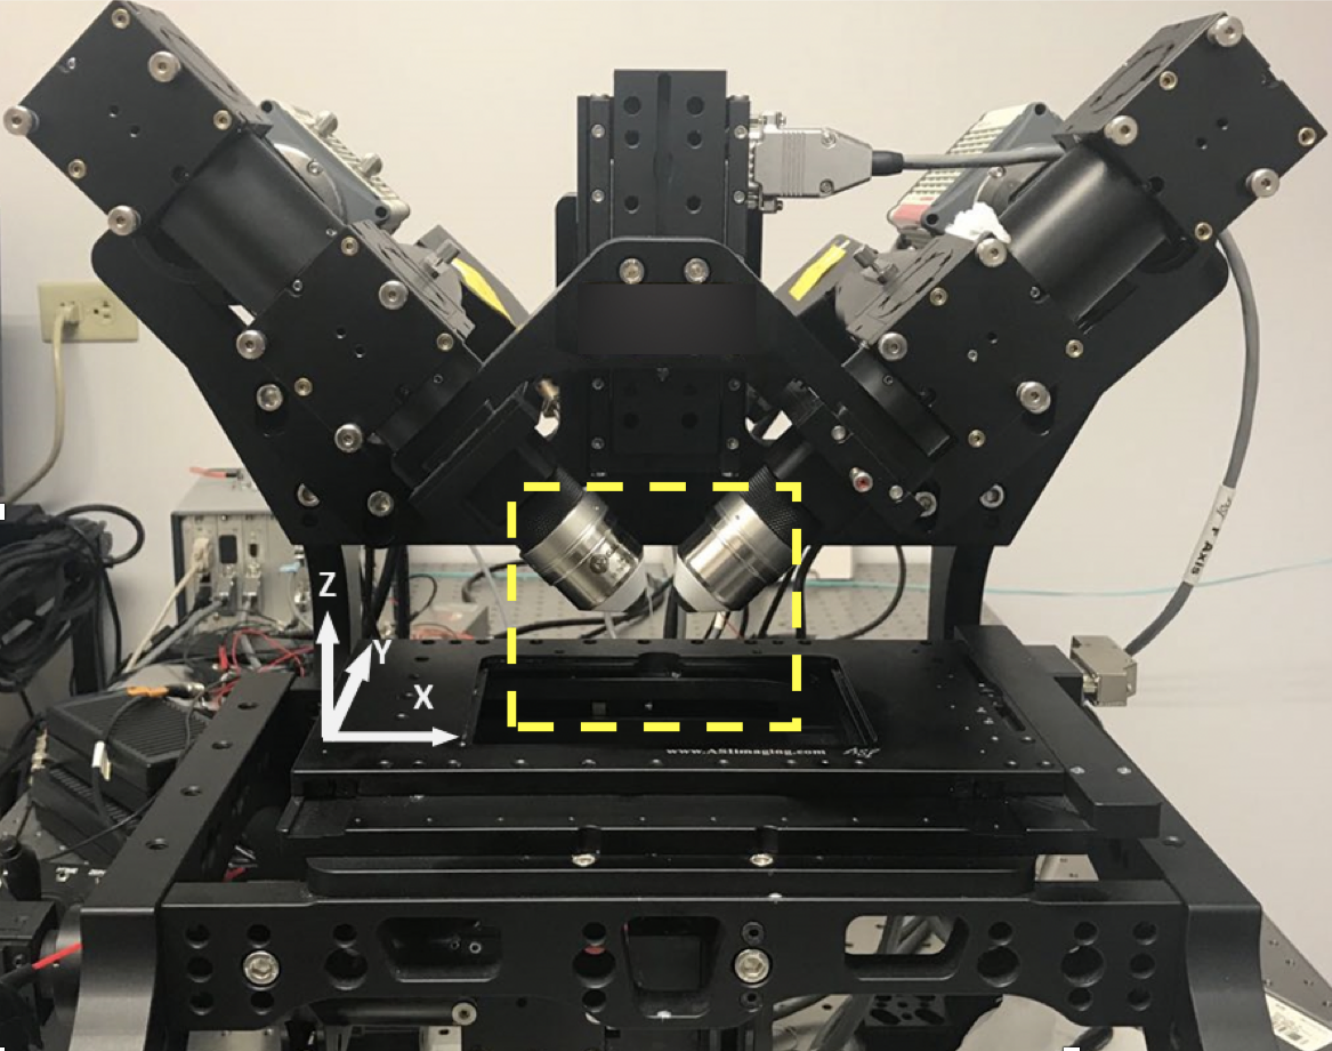
\includegraphics[width=0.5\linewidth]{./img/lsm_device_02.png}
				\caption{Le microscope \textit{diSPIM} conçu par les chercheurs de la Nouvelle Orléans permettant une acquisition tridimensionnelle d'un échantillon de manière fiable et rapide}
				\label{lsm_02_device}
			\end{figure}

			Dans leur dispositif d'acquisition d'images, il existe donc deux dispositifs \textit{SPIM} qui servent tour à tour de capteur, puis d'émetteur. Ces deux dispositifs sont placés à angle droit l'un de l'autre (voir \ref{lsm_02_device}), au dessus de la plateforme sur laquelle on dépose l'échantillon transparisé à analyser. Le fait d'avoir deux dispositifs \textit{SPIM} permet de se ramener à une acquisition 3D à résolution isotropique\footnotemark~ en combinant les acquisitions des capteurs avec leurs points de vue différents.\\
			\footnotetext{Inverse d'anisotropie : les propriétés sont les mêmes dans toutes directions}
		}
		\section{Particularités du microscope}\label{section:02_02_microscope}
		{
			La méthode \textit{LSFM} (plus particulièrement, la méthode \textit{SPIM}) fut choisie pour sa résolution de l'ordre du micromètre, par sa rapidité relative d'acquisition par rapport à d'autres méthodes, et par sa capacité à effectuer de l'imagerie 3D aisément dans un milieu transparent. Malgré cela, il existe un désavantage à cette méthode : dû au fait que l'acquisition se fait par détection de lumière dans le milieu à analyser, l'image devient de moins en moins nette au fur et à mesure que l'on s'éloigne de la source de lumière.\\
			Afin de pallier à ce problème, les chercheurs de l'université de Tulane ont choisi de concevoir un microscope en utilisant deux dispositifs \textit{SPIM} (voir figure \ref{lsm_02_device}). Ce dispositif leur permet donc de pallier au problème induit par la diffraction de la lumière, mais ne résout pas entièrement le problème de netteté de la prise de vue. Il faut déconvolutionner\footnotemark les deux images, une fois traitées afin d'obtenir une grille représentant réellement l'échantillon acquis.
			\footnotetext{La déconvolution est un procédé algorithmique mathématique visant à améliorer la qualité d'un signal enregistré. Ici, les images acquises par le microscope}
		}
		\section{Motivation de la méthode}\label{section:02_03_motivation}
		{
			À l'heure actuelle, les diagnostics du cancer de la prostate sont effectués grâce à des coupes histologiques d'un échantillon de prostate d'un patient. La forme des glandes dans le tissu est ensuite comparé de manière empirique à une échelle qualitative appelée échelle de Gleason~\cite{cite_gleason_score} (voir figure \ref{gleason_score}), donnant un diagnostic permettant de savoir si un patient a besoin d'être traité ou non.\\

			\begin{figure}[!htp]
				\centering
				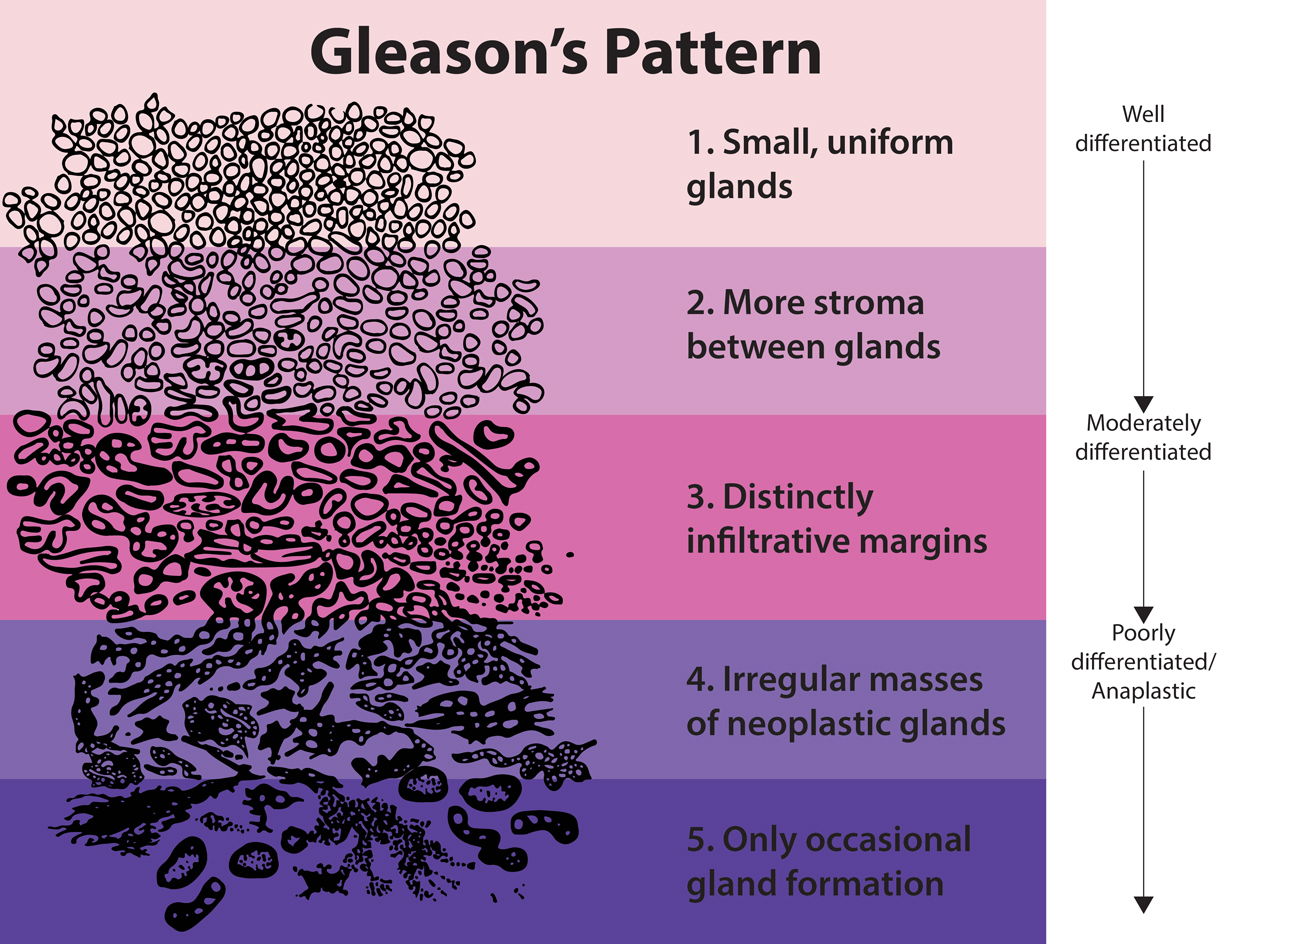
\includegraphics[width=0.5\linewidth]{./img/gleason_score.jpg}
				\caption{Le score de Gleason, permettant une approximation de l'avancement du cancer de la prostate par l'appréciation visuelle de la forme des glandes de celle-ci}
				\label{gleason_score}
			\end{figure}

			Malheureusement, étant une méthode de diagnostic basée sur une observation empirique, cette méthode possède ses fautes. Par exemple, l'orientation de la coupe histologique dans l'échantillon de tissu du patient importe beaucoup sur la forme finale des glandes observées, ce qui peut mener à une erreur dans le diagnostic du patient. Cette faiblesse de la méthode de Gleason est la raison principale pour laquelle il est important d'avoir une nouvelle méthode d'analyse tridimensionnelle de la prostate. Grâce à cette nouvelle approche, il serait ainsi possible de développer une nouvelle méthode de diagnostic du cancer de la prostate reposant sur la forme tridimensionnelle des glandes, et non sur une coupe 2D qui pourrait entraîner des mauvais diagnostics.\\
		}

	}

	\chapter{Problématique de stage}\label{section:03_stage_problematique}
	{
		\section{Méthode actuelle}\label{section:03_01_methode_actuelle}
		{
			Afin d'obtenir quelques résultats préliminaires de leur microscope, les chercheurs de l'université de Tulane ont conçu une simple méthode de reconstruction. Cette méthode leur permet, après un temps de calcul considérable, d'obtenir une approximation de la reconstruction tridimensionnelle de l'échantillon acquis.\\

			Malheureusement, la méthode utilisée possède des défauts. Elle ne prend pas en compte les spécificités du microscope, et prend un temps et un espace mémoire conséquents. Cette méthode aboutit à une grille non exploitable, car celle-ci est trop grande pour être confortablement chargée en mémoire.\\

			Leur microscope donne, en fin d'acquisition, deux piles d'images prises à 90 degrés l'une de l'autre, selon l'orientation de leurs capteurs (voir figure \ref{lsm_02_device}). Ces deux piles sont toutes les deux nécessaires pour reconstruire le modèle, car il faut effectuer une étape de déconvolution des images afin d'améliorer la netteté de l'acquisition, comme discuté précédemment.\\

			\begin{figure}[h]
				\centering
				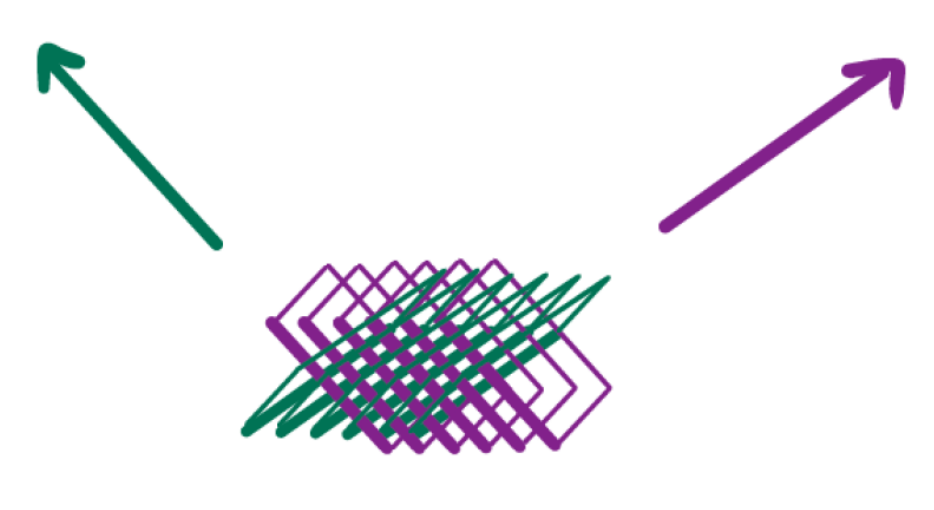
\includegraphics[width=0.5\linewidth]{./img/tulane_reconstruction_04_image_stacks.png}
				\caption{Visualisation des deux piles d'images en sortie du microscope. Une pile (violette) est prise par le capteur de gauche, et une autre pile (verte) est prise par le capteur de droite. Grâce aux deux acquisitions, on peut se ramener à une capture isotropique de l'échantillon}
				\label{img:tulane_04_img_stacks}
			\end{figure}

			Leur méthode consiste à effectuer une reconstruction de l'échantillon en six étapes :

			\begin{enumerate}
				\item Pour la pile 1 (un résumé visuel est disponible en figure \ref{ref_tulane_recon_01_shift_up}) :
				\begin{enumerate}
					\item Redimensionnement des pixels en voxels\footnotemark (afin de passer d'une pile de photos à une grille 3D)
					\item Itérer sur des ensembles de voxels (soit une ligne dans toutes les images, soit une colonne dans toutes les images) afin de les transformer en images 2D, en rééchantillonnant trilinéairement les images afin d'avoir plus de résolution
					\item \label{itm:wrong_shift}Décalage, rotation et mise à l'échelle des images résultantes afin d'obtenir la vraie forme de l'échantillon lorsqu'il fut acquis
					\item Itération sur toutes les images 2D obtenues précedemment, et les réinterpoler afin d'obtenir une grille 3D
				\end{enumerate}
				\item Répéter toutes les opérations de la pile 1 sur la pile 2
				\item Utiliser les informations des deux grilles afin d'effectuer une déconvolution du signal, améliorant la netteté de la grille résultante
			\end{enumerate}
			\footnotetext{Pixel = \textbf{Pi}cture \textbf{El}ement, Voxel = \textbf{Vo}lumetric \textbf{El}ement}

			\begin{figure}[h]
				\centering
				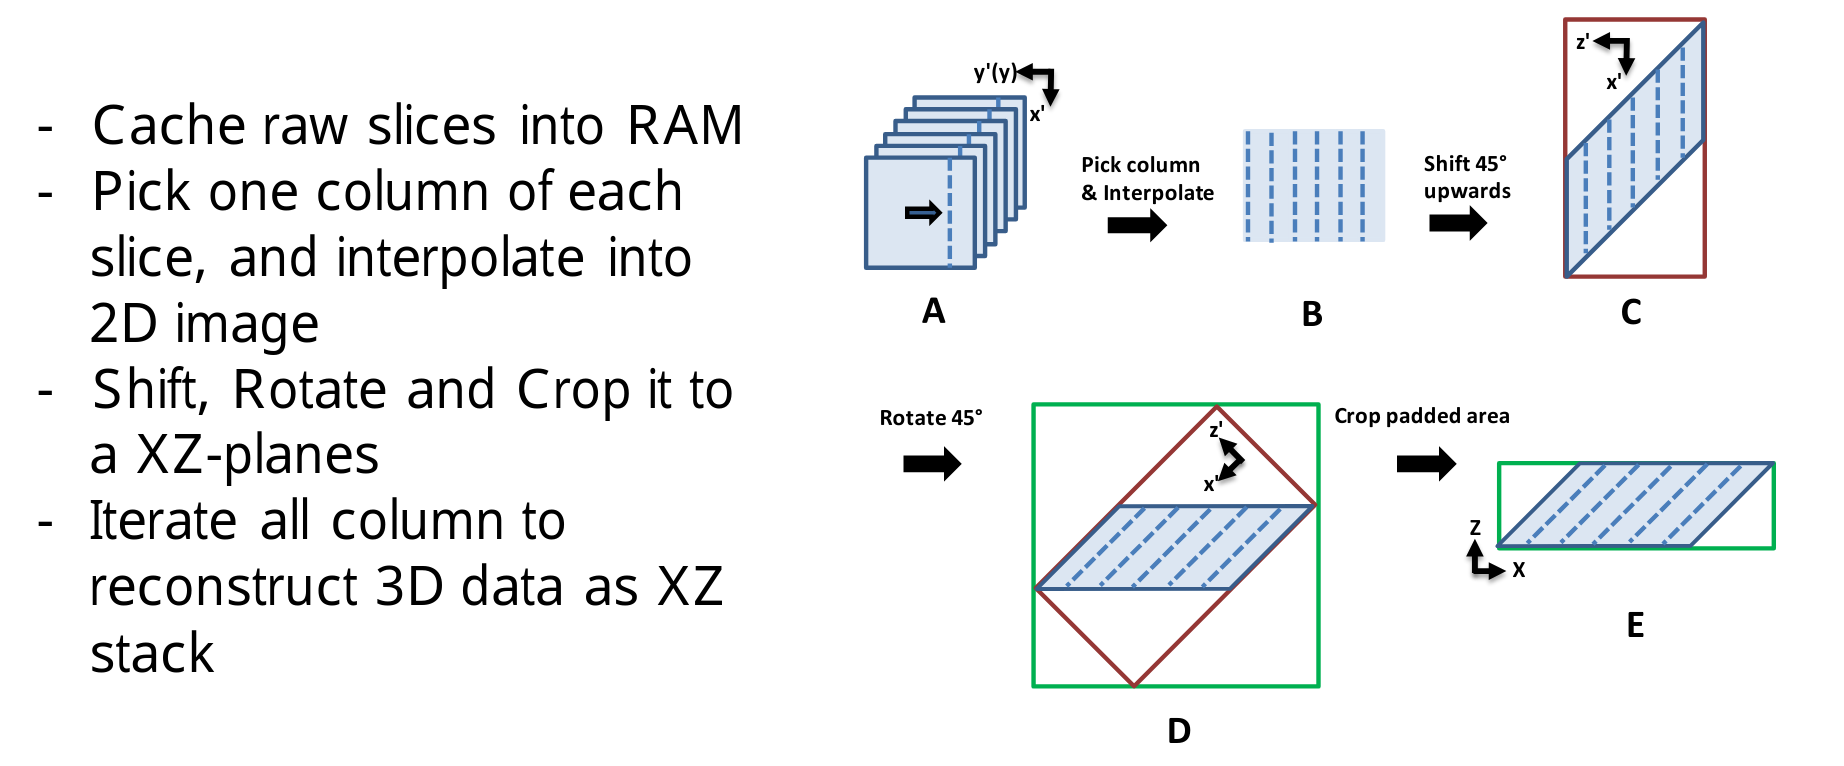
\includegraphics[width=0.8\linewidth]{./img/tulane_reconstruction_01_shift_up.png}
				\caption{Méthode de reconstruction d'une pile d'images en une grille de voxels, conçue par les chercheurs de l'université de Tulane}
				\label{ref_tulane_recon_01_shift_up}
			\end{figure}

			Cette méthode est actuellement en utilisation pour le développement de leur microscope, et est un majeur problème au développement de ce dernier dû au temps et à l'espace mémoire pris. Un autre problème non négligeable de la méthode est que la transformation effectuée dans l'étape \ref{itm:wrong_shift} pour émuler la forme des prises de vues dans l'échantillon n'est pas exacte. Elle ne reproduit pas exactement le contenu de l'échantillon, étant donné que les prises de vues le représentant ont d'abord étés rééchantillonnées avant d'être manipulées ou déplacées.
			Par exemple, voici une des reconstructions qu'ils ont effectuées sur un échantillon de tissu de sein humain :

			\begin{figure}[H]
				\centering
				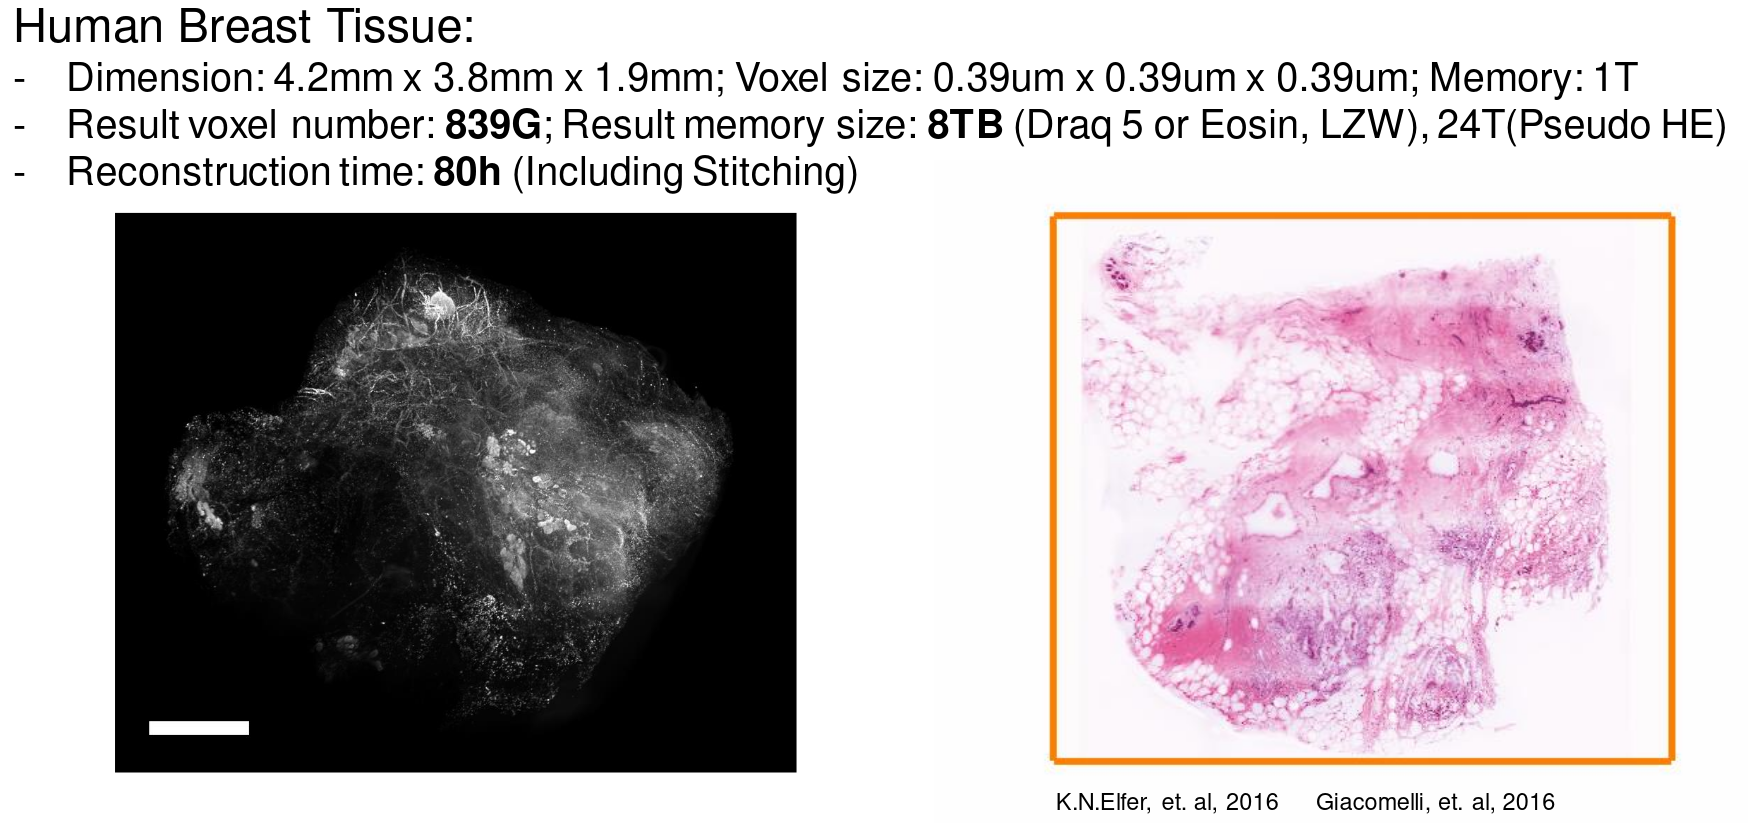
\includegraphics[width=0.8\linewidth]{./img/tulane_reconstruction_02_breast.png}
				\caption{Exemple de reconstruction d'un échantillon de tissu humain avec la méthode actuellement en place à Tulane}
				\label{ref_tulane_recon_02_breast}
			\end{figure}

			Pour une acquisition d'un échantillon de environ $30\text{mm}^3$, il leur a fallu non seulement 1 téraoctet de mémoire, mais aussi plus de 80 heures de traitement, pour aboutir à une grille de plus de 8 téraoctets. Un changement de méthode s'impose donc, car si ces acquisitions ne peuvent pas être vues par un médecin dû à la taille énorme des grilles résultantes, le microscope ne servirait à rien.\\

			Parmi les nombreux problèmes de cette méthode, le plus important est la quantité massive de données créées afin de reconstruire une image tridimensionnelle de l'échantillon acquis. En effet, une fois l'image 3D obtenue, il faut ensuite qu'un médecin puisse la manipuler afin de produire un diagnostic, il faudrait donc que la quantité de données résultante de la reconstruction 3D soit capable d'être gérée par tous types d'ordinateurs, peu importe leur âge. En effet, leur méthode produit aussi beaucoup d'espace vide, prenons par exemple cette reconstruction de tissu de prostate humaine :

			\begin{figure}[H]
				\centering
				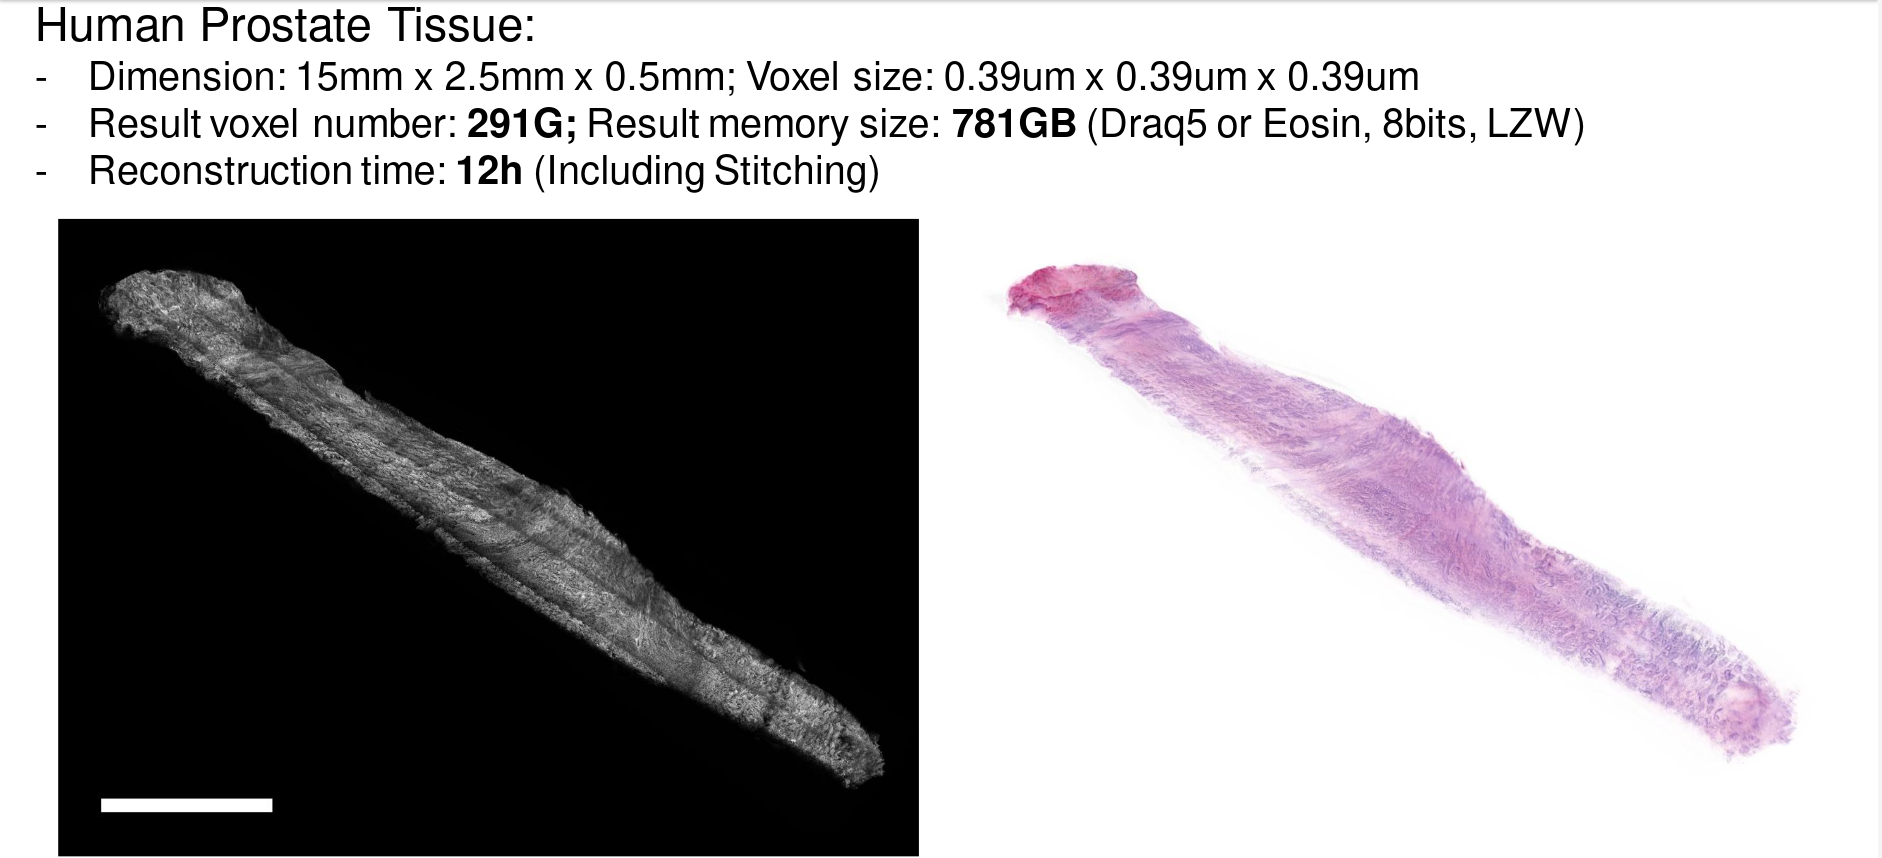
\includegraphics[width=0.8\linewidth]{./img/tulane_reconstruction_03_prostate.png}
				\caption{Imagerie de la prostate reconstruite en 3D, contenant beaucoup d'espace vide autour de l'échantillon}
				\label{ref_tulane_recon_03_prostate}
			\end{figure}

			On peut voir que cette reconstruction possède une grande partie de ses données dédiées à afficher de l'absence d'information, ce qui allourdit le fichier résultant inutilement, et qui rallonge artificiellement le temps de traitement.\\

			L'un des objectifs premiers serait donc de pouvoir trouver une méthode de reconstruction tridimensionnelle permettant de reconstruire les échantillons plus rapidement, en utilisant moins d'espace mémoire et en prenant en compte les spécificités du microscope.
		}
		\section{Visualisation des grilles de voxels}\label{section:03_02_solution}
		{
			L'un des objectifs principaux du stage reste quand même la visualisation interactive des grilles résultantes. Une fois les acquisitions d'échantillons reconstruites en trois dimensions, il faudra donc trouver une méthode de visualisation afin de les manipuler en temps réel.\\

			Un premier point de départ serait d'effectuer une vue en multi-résolution de la grille. Par exemple, le système de \textit{QSplat}~\cite{cite_visu_qsplat_system} de Rusinskiewi qui permet d'afficher un modèle interactivement en utilisant une arborescence de "vue" du modèle. Cela nous permettrait d'avoir une vue interactive, avec plus de détails ajoutés lorsque l'utilisateur ne manipule pas le modèle.

			On pourrait aussi effectuer une visualisation avec régions d'intérêt, soit définies manuellement, soit selon un critère défini sur le modèle. De cette façon, l'utilisateur pourrait choisir quelles régions ont besoin d'avoir plus de détail, afin de pouvoir analyser une partie spécifique de l'échantillon acquis.
		}
		\section{Travaux supplémentaires}
		{
			En parallèle de ce sujet de stage, j'ai fourni mon aide à Mme \textsc{Faraj} sur un projet de visualisation de grille de voxels. Ce travail sera soumis à la prochaine conférence IEEE Vis, qui se tiendra dans le courant de l'automne 2020.\\

			Ce projet permettrait une visualisation interactive de grilles de plusieurs milliards d'éléments interactivement. De plus, cela nous permettrait de faire des plans de coupe afin que les médecins qui se servent de ce programme puissent voir le modèle sous plusieurs angles, ainsi que d'effectuer des coupes histologiques si ils le souhaitent.\\

			Ce travail, ayant pris la majorité du temps de stage jusqu'à maintenant, peut servir de point de départ pour la partie visualisation une fois que la reconstruction tridimensionnelle sera finie.
		}
	}

	\selectlanguage{french}
	\bibliography{references}{}
	\bibliographystyle{plain}
\end{document}

% VIM modeline : do not touch !
% vim: set spell spelllang=fr :
